% !TeX spellcheck = en_US
\label{sec:results}

Using the concept, described in Chapter \ref{sec:concept}, I was able to implement the newly designed parts of the ER model, shown in Figure \ref{fig:db-er-model}, in the \masymos \neoj stack. These graph structures are generated by a plugin written to interface the native \neoj API on the one side and \bives on the other.
Converting this formal described ER model into a graph database schema as shown in Figure \ref{fig:results:simple-diff}, was performed as described in Section \ref{sec:background:graph-db:er}. Despite the direct convertibility, some optimizations and adjustments for convenience were made, like introducing the common label \texttt{DIFF\_NODE} for all change types.
Also the figure shows a simplified representation of a delta between two versions of a relatively simple toy model. The figure was reduced to maintain readability, while still illustrating the basic schema.

The schema was designed around a \texttt{DIFF} node, which is linked by \texttt{HAS\_DIFF} relations, from two consecutive versions of the same model. These two versions are again linked with the \texttt{HAS\_SUCCESSOR} and \texttt{HAS\_PREDECESSOR} relations.
The successor and predecessor relations define the version history, whereby the \texttt{DIFF} node clearly indicates the delta between those versions. The \texttt{diffPart} attribute of the \texttt{HAS\_DIFF} relations specifies the direction of the delta, and therefore the role of the participating \texttt{DOCUMENT} nodes. In accordance to the ER model, the role can either be \emph{source} or \emph{destination}.
These terms were chosen, due to their expressiveness in regards to temporal aspects. Otherwise an implication of order, like terms as \emph{old} and \emph{new} suggest, may cause confusion in case of reverse deltas or deltas between completely different models.

However, the central \texttt{DIFF} node links to various changes, using the\linebreak \texttt{HAS\_DIFF\_ENTRY} relation. Since \neoj supports multiple labels per node, the 4 change types \texttt{DIFF\_INSERT}, \texttt{DIFF\_DELETE}, \texttt{DIFF\_UPDATE}, and \texttt{DIFF\_MOVE} can be grouped together using an additional label \texttt{DIFF\_NODE}. This simplifies queries and will eventually speed them up, because all change types are kept in a single index.
Any kind of \texttt{DIFF\_NODE} might link to any node beneath the \texttt{DOCUMENT} node in at least one of the two compared models, in correspondence to the type of change.
As illustrated by the \texttt{DIFF\_UPDATE} node in Figure \ref{fig:results:simple-diff} (small yellow node, labeled with a \emph{2}). On one hand it connects to the species \emph{A} in the \emph{source} version of the model using the \texttt{IS\_SOURCE} relation. On the other hand it also connects to the updated counterpart in this case species \emph{A} in the \emph{destination} version. It is connected using the \texttt{IS\_DESTINATION} relation.
Furthermore a causality chain among changes is expressed by the \texttt{DIFF\_TRIGGERED\_BY} relation, which points from one \texttt{DIFF\_NODE} to another. This is illustrated by the \texttt{DIFF\_INSERT}, labeled with the number \emph{3}, in Figure \ref{fig:results:simple-diff}. This insert caused four other inserts, describing the insertion of id, name, compartment reference, and initial concentration.

In addition to these structural information each \texttt{DIFF\_NODE} contains all attributes \bives assigns to a change. These \bives specific information include an XPath expressions, name, and id of the changed \xml element. All these attributes can be used together, to locate the change in both versions.
Further the nodes includes the values of \emph{source} and \emph{destination} in case of an attribute change, as well as a possible reference to another change, that triggered this current one.
Besides the \bives attributes, the \texttt{DIFF\_NODE} also contains an \texttt{inherit} flag. It indicates, if a change detected by \bives, does not have a direct match in \masymos's graph structure. Instead the model structure is traversed upwards, until an element is found, which has a representation in the \masymos graph.
This, for instance, applies to changes of a mathematical parameter in a kinetic law of a reaction. In this specific example, the change would be linked to the node representing the reaction, since mathematical structures or kinetic laws are not represented in \masymos. Another example would be text nodes of any kind, which are stored within a Lucene index by \masymos, but not in the graph representation, since they are not an essential part of the models structure.
The \texttt{inherit} flag consequently allows to store and analyze changes, which otherwise could not be integrated into the schema.

Furthermore \texttt{DIFF\_NODE} nodes might link to multiple \comodi terms, whereby \comodi's own relationship names are used, instead of the generic \texttt{is\_a} link, proposed in the concept Section \ref{sec:concept:dbmodel}.
Further \comodi's entire reasoned taxonomy is stored in \masymos, so queries matched against abstract terms also include references to more specialized terms. The resulting network is shown in Appendix \ref{fig:appendix:neo4j-comodi}.
Before generating any deltas the \comodi ontology needs to be imported initially. Otherwise terms might be created on occurrence, but not interlinked according to the taxonomy.
The initial import is performed using already existing mechanisms in \masymos, which were only adjusted, so they can handle dynamic ontology names (cf. Section \ref{sec:impl:masymos}). In this process the ontology is first loaded in its \owl representation and then validated with the Hermit reasoner \citep{Shearer2008}. The second step does not only makes sure that only logically correct ontologies are imported, but also to imports \emph{inferred} ontologies. This moves the logical classification step from querying to the import of ontologies.
A graphical and tabular overview of all used node labels and relation types can be found in Appendix \ref{sec:appendix:meta-map}.

The import of actual models, however, is performed by the \modelcrawler (cf. Section \ref{sec:impl:modelcrawler}), resulting in a \masymos database filled with all model versions of \emph{BioModels Database} and \emph{PMR2} (cf. Section \ref{sec:background:modelrepo}) and a hierarchical file structure containing all original files, complying with the model described in Section \ref{sec:concept:filestorage}.
During a test run from 2016-10-14, this resulted in a dataset with $3367$ distinct models and  $14503$ model versions, with $4.307$ versions per model on average. The accumulated test data consumes $8.5$ GBytes of disc storage for the database, excluding the cached original files (cf. Section \ref{sec:concept:filestorage}).
This data was gathered from all publicly available workspaces in \emph{PMR2} and all releases of the \emph{BioModels database} (cf. Section \ref{sec:background:modelrepo}) using the \modelcrawler (cf. Section \ref{sec:impl:modelcrawler}).
\todo{point to appendix, explaining how the import was done}

On the contrary, models for test purposes and to generate Figure \ref{fig:results:simple-diff} were imported using a small Python\footnote{\url{https://www.python.org/}} script. This script emulates a HTTP daemon, while simultaneously sending import commands to the \masymos \rest interface \morre. It eases the process of importing test data, since neither the \modelcrawler needs to be configure, nor a sane folder structure needs to be built manually.

In conclusion, the extension of the \masymos database allows to store, access, query, and compare multiple versions of biological models, enriched by semantical annotations. Whereas the extended \masymos database is providing an efficient index for a variety of structural, textual and semantic aspects, the original files are still available in the filesystem.
This attempt combines benefits from both approaches.
On one hand the indexed graph database provides excellent analytical features while maintaining reasonable performance. On the other hand it ensures the exact reproduction of the original model files.
Overall this solution meets the requirements set by \citet{Waltemath2013}, that a good "model VCS should be tailored to existing model  representation formats, which are typically XML and RDF based. It should furthermore reflect the temporal evolution of a model and present model changes to the users" \citep{Waltemath2013}.

 
\begin{comment}
\todo{what's done from the concept}
\todo{still high-level}
\todo{what problem is solved?}

\begin{itemize}
	\item implemented db concept
		\subitem picture from simple-sbml-demo
		\subitem rest of pictures in appendix
	\item Ontology import
		\subitem changes to \masymos core
		\subitem using existing import mechanics, but dynamic
	\item http server storage concept?
\end{itemize}

solved:
"A model VCS should be tailored to existing model representation formats, which are typically XML and RDF based. It should furthermore reflect the temporal evolution of a model and present model changes to the users." \citep{Waltemath2013}

The objective of this thesis is therefore to investigate into a concept to store systems biology models in a way, that multiple versions can be accessed, queried, and compared. Further, semantical annotations of changes between these versions shall be introduced. These additional relations are meant to improve the ability to query for a version of a model by specific criteria and consequently improving the user experience for biologists seeking to build onto existing models, as the evolution of them plays an important role for them \citep{Scharm2015}
\end{comment}

\begin{figure}
	\centering
	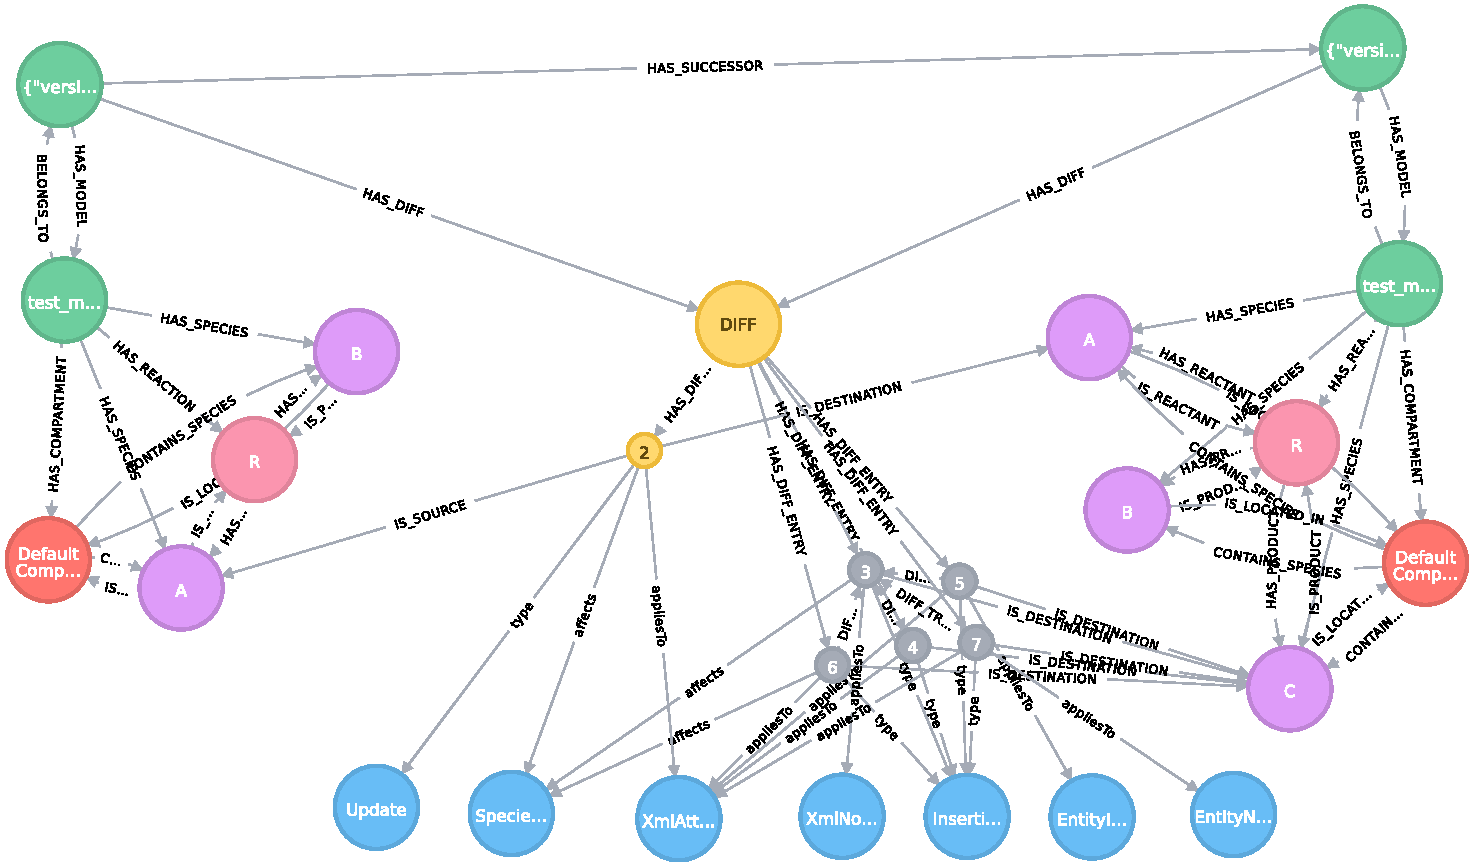
\includegraphics[width=\textwidth]{resources/neo4j-renders/demo-sbml-simple-diff.pdf}
	\caption[Reduced representation of a delta in \masymos, between two versions of a the simple \sbml demo model]{Reduced representation of a delta in \masymos, between two versions of a the simple \sbml demo model. The delta, organized around the \texttt{DIFF} node, only shows changes, with a direct match in the graph representation. Further most up traversing relations are not shown, to increase readability.}
	\label{fig:results:simple-diff}
	\todo{show \comodi as ontology}
	\todo{Make relation names readable}
	\todo{colorize the different diff nodes}
\end{figure}